\chapter{Phase 1: Spezifikation und Grob-Design}

\section{Use Case Diagram}
Da in der ersten Phase des Systementwurfs die elementaren Funktionen der Smartwatch, sowie die Anwendungszwecke identifiziert werden mussten, erfolgt eine grobe Beschreibung dieser Funktionen mithilfe von Use Case Diagrammen. Zum Zeitpunkt des ersten Systementwurfs war die Festlegung auf Hardware-Komponenten noch nicht final. Daher beschränken sich die ersten Use Cases ausschließlich auf elementare Basisfunktionen der Smartwatch: Anrufe, Fitness und Pairing.


\begin{figure}[H]
\centering\
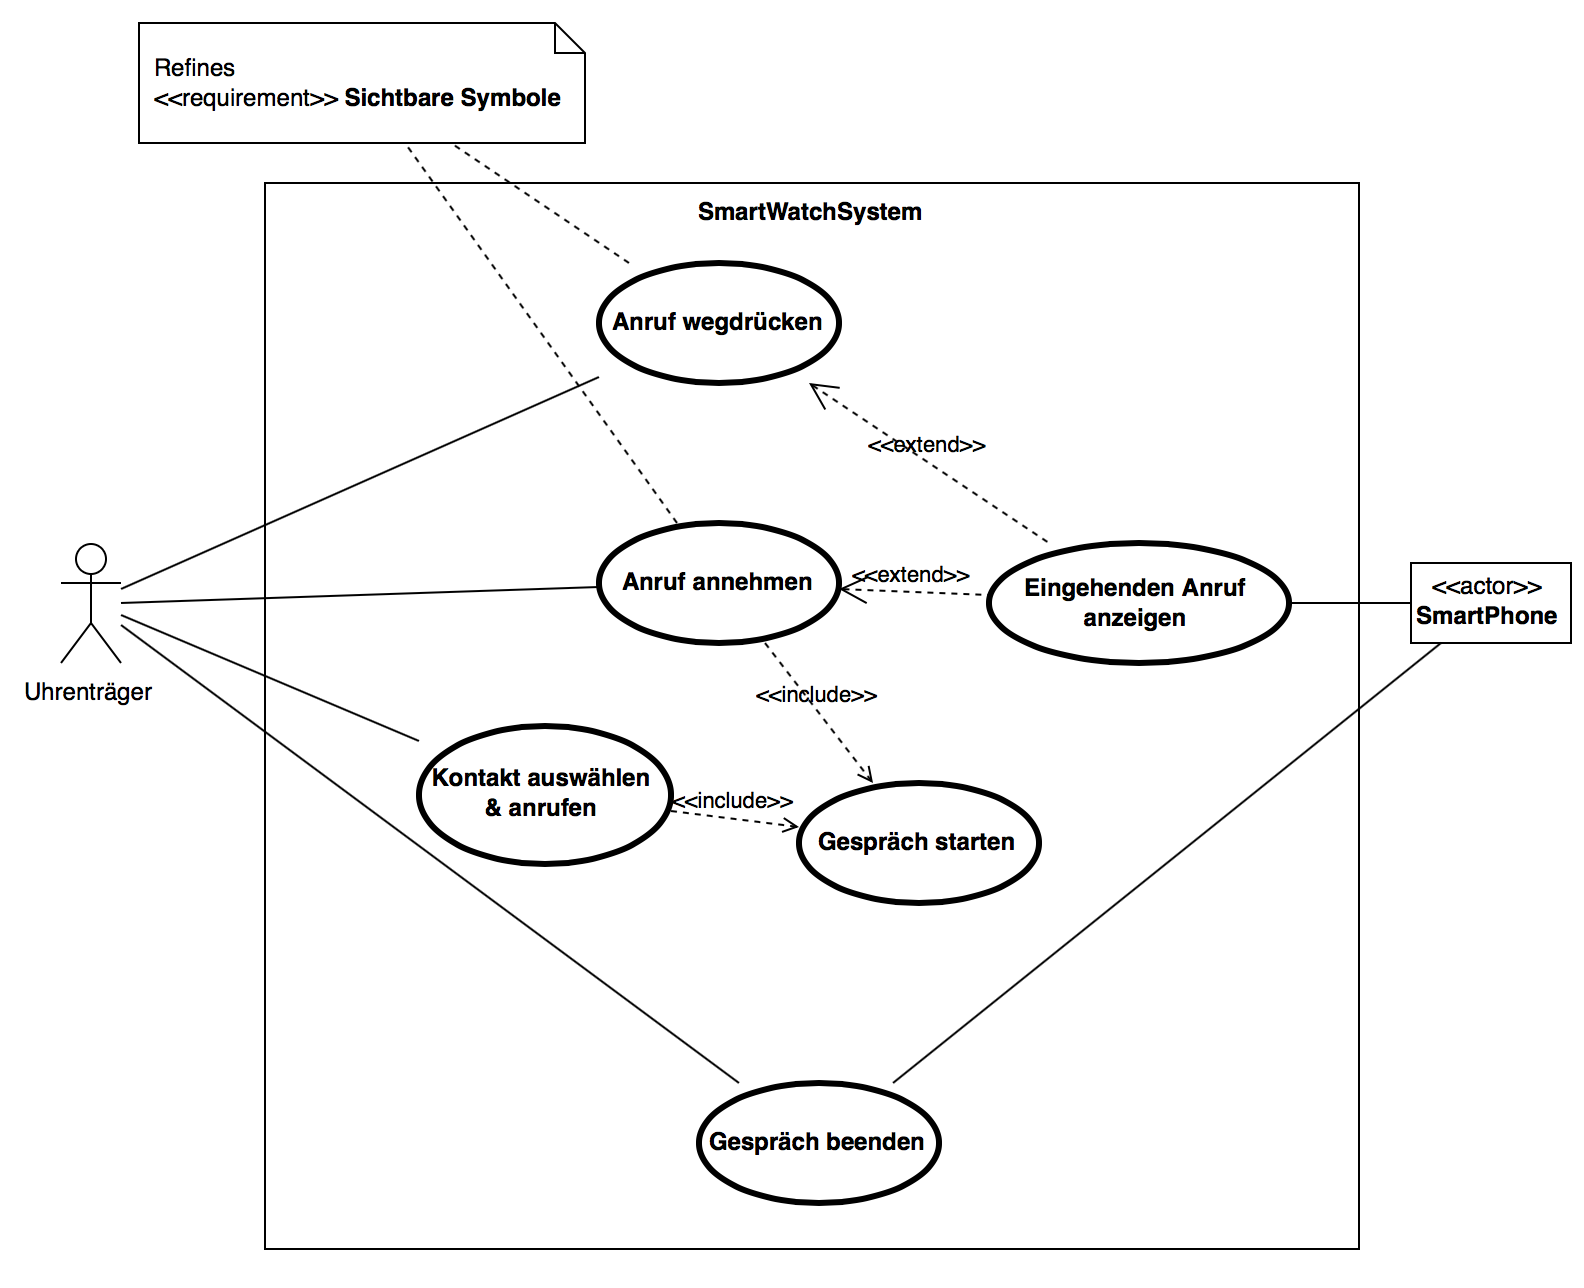
\includegraphics[width=14cm]{img/usecase-anruf-p1}
\caption{Use Case - Anruf}\label{fig:usecase-anruf-p1}
\end{figure}

\begin{figure}[H]
\centering\
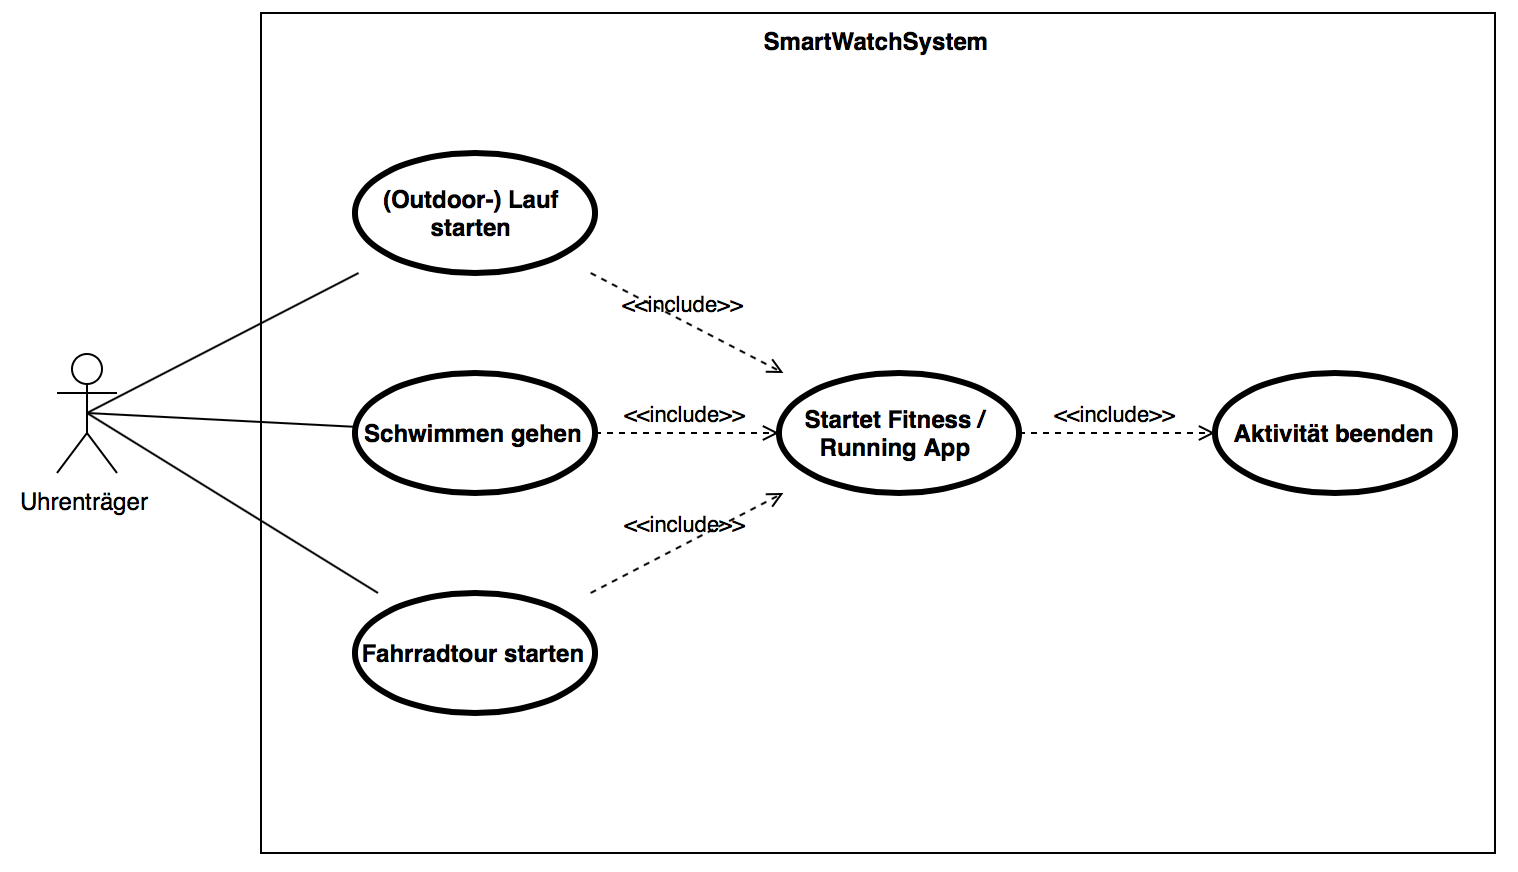
\includegraphics[width=14cm]{img/usecase-fitness-p1}
\caption{Use Case - Fitness}\label{fig:usecase-fitness-p1}
\end{figure}

\begin{figure}[H]
\centering\
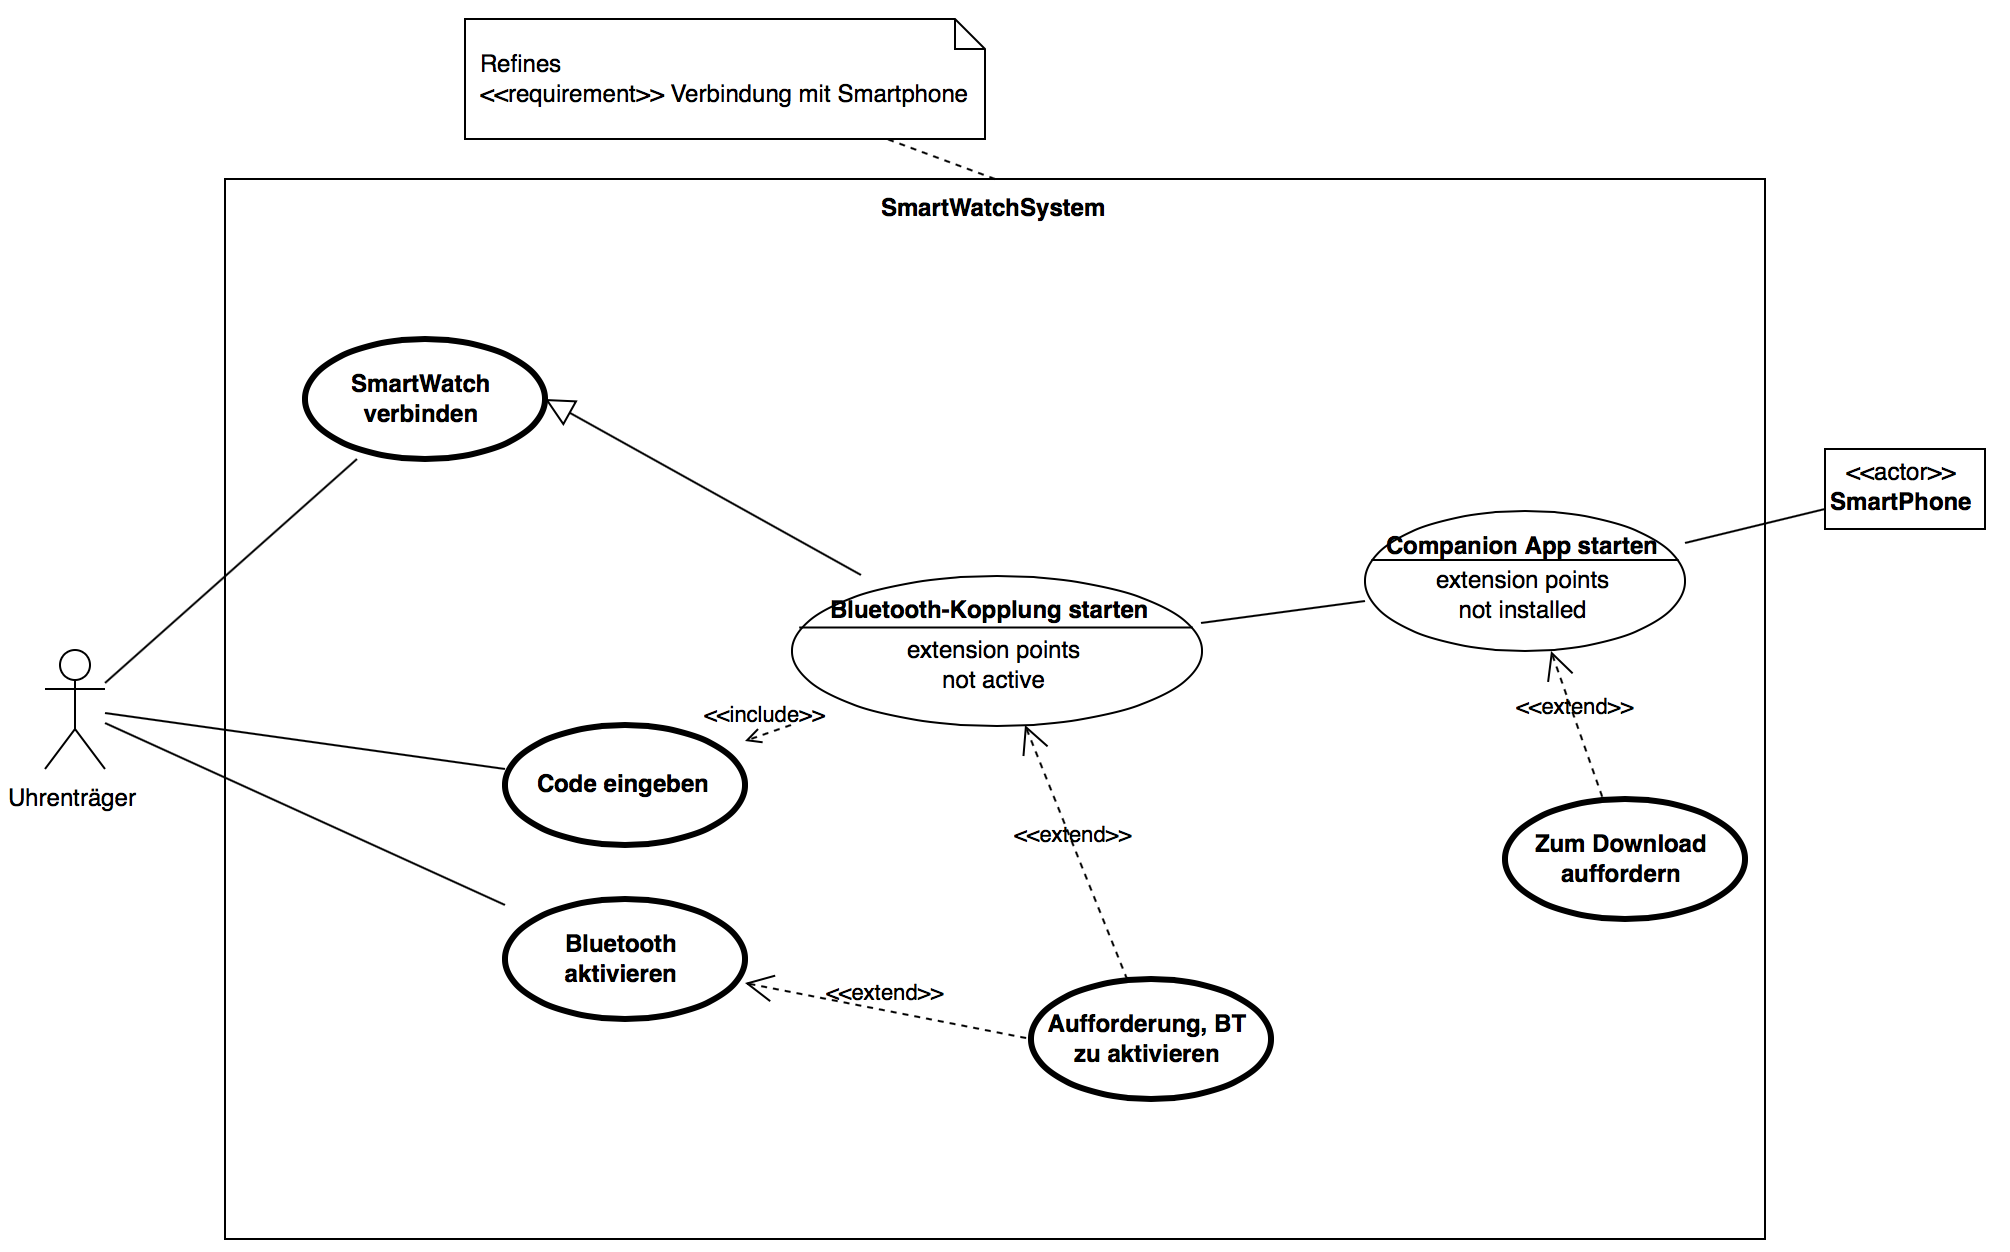
\includegraphics[width=14cm]{img/usecase-pairing-p1}
\caption{Use Case - Pairing}\label{fig:usecase-pairing-p1}
\end{figure}

\section{Requirement Diagram}

\section{Package Diagram}
Um die Struktur des Smartwatches zu gliedern und so Schichten in verschieden Abstraktionen
einzuführen werden Paketdiagramme verwendet.
Der Smartwatch wurde dabei in funktionalen und logischen Einheiten zerlegt und in dem jeweiligen Paket zugeordnet.
Über die rein funktionalen Eigenschaften des Systems werden auch die nicht-funktionalen Anforderungen des Smartwatches in Pakete definiert.


Die Abbildung ~\ref{fig:package} beschreibt die Pakete des Smartwatches.
\begin{figure}[H]
\centering\
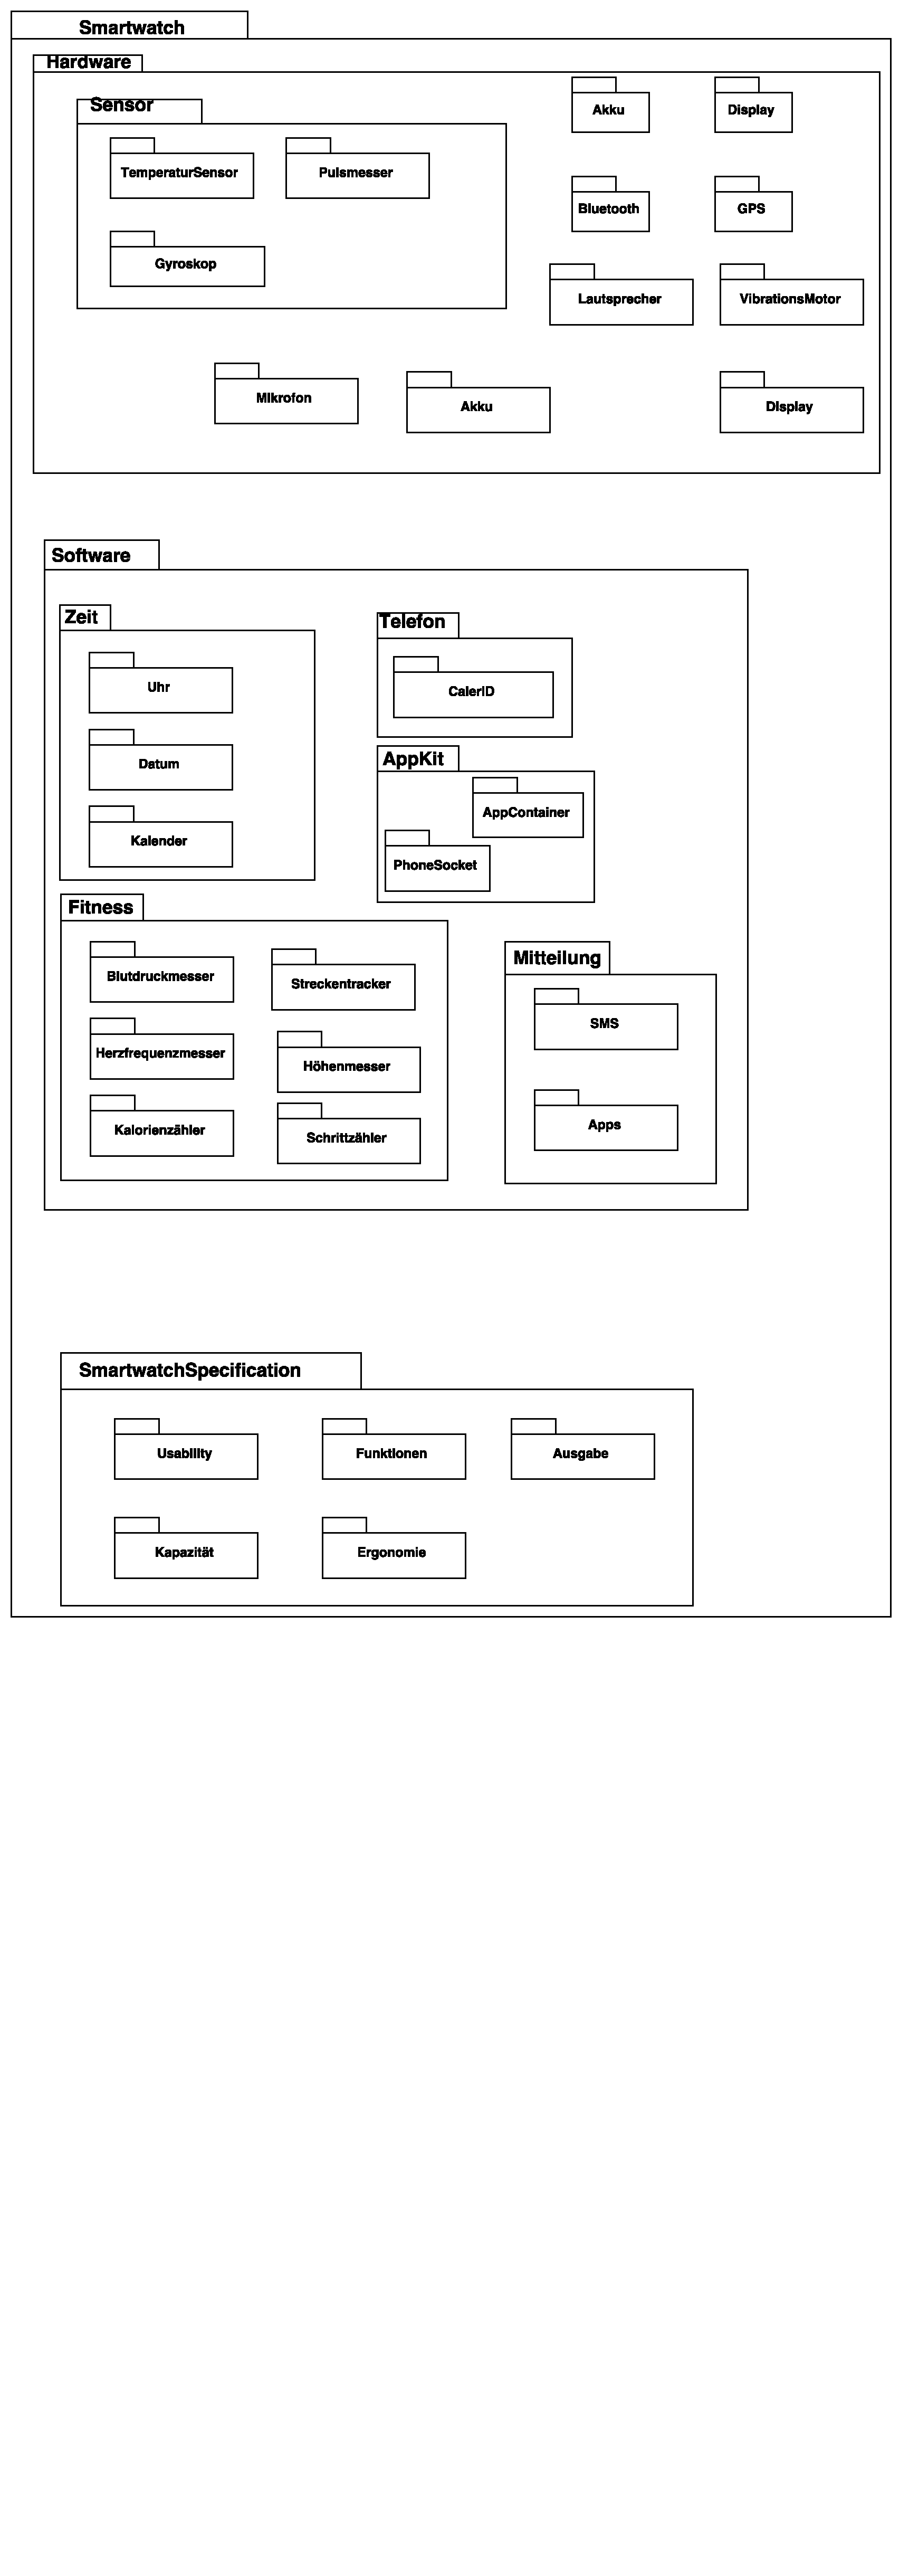
\includegraphics[width=8cm]{img/package}
\caption{Packetdiagramm}\label{fig:package}
\end{figure}

Die Elemente des Pakets Smartwatch sind wiederum Pakete, welche die verschiedenen funktionalen Zuständigkeiten innerhalb des Pakets SmartWatch beschreiben.
Der Smartwatch-Paket ist in Hardware, Software und den nicht-funktionalen Anforderungen
gegliedert (\textit{SmartWatchSpecification}).
Für die Verbindung sorgt Bluetooth 4.0. 
Als Sensoren kommen ein Schrittzähler, ein Pulsmesser, Temperatursensor und Gyroskop zum Einsatz. Für die Verbindung sorgt Bluetooth 4.0. 
Die Sensoren können z.B zur Aktivitätserkennung.
Der Smartwatch besitz ein Display, auf dem dann wichtige Infos wie Anrufernummer und Benachrichtigungen und die Uhrzeit angezeigt werden.
Die weiteren Hardwarebausteine sind im Package \textit{Hardware} zu finden.

Standard Anwendungen die mit dem Smartwatch geliefert werden, sind Uhrzeitangaben, Erinnerungsfunktionen, Kalender Funktionalität, Benachrichtigungen oder die Aktivitätserkennung. Klassische Anwendungen sind auch die Fitnessfunktionalitäten.
Mit der mitegelieferten API \textit{AppKit} lassen sich Apps für die SmartWatch programmieren, die eng mit dem Smartpohone zusammenarbeiten. 
Die softwaretechnische Paketstruktur ist im Package \textit{Software} abgebildet.

\section{Block Definition Diagram !!!Nochmal durchlesen!!!überarbeiten!!! auf die Values der Blocks eingehen!!!}
Das Blockdefinitionsdiagramm !!!Verweis auf Anhang!!! in dieser Phase stellt den groben, physikalischen Aufbau der Smartwatch dar. Diese setzt sich zusammen aus Sensoren, einem Display, einem Speichermedium, einem Armband, einen Gyroskop, einer Bluetooth-Antenne und einem GPS-Modul. Um die Stromversorgung der Uhr zu garantieren, soll das Armband aus mehreren Akkuzellen bestehen. Das Display soll dabei komplett von der Uhr trennbar sein. So kann die Uhr bei schwachen Akku oder bei einem Wechsel zu einer sportlichen Tätigkeit einfach in einem anderen Armband eingesetzt werden. Die Bluetooth-Antenne soll die Verbindungsstelle zum Smartphone sein. Um die Akkulaufzeit zu erhöhen soll die Antenne, zusätzlich zum normalen Bluetooth, auch "Low-Energy" -Bluetooth unterstützen. Die Smartwatch selbst soll keine Daten, außer die für die Nutzung reiner Sportaktivitäten benötigten, speichern können. Daher ist der Speicher recht klein gehalten und dient nicht zum verwalten von Bildern oder anderen Benutzerdaten. 
Zu diesem Zeitpunkt der Entwicklung waren die Funktionalitäten noch nicht fertig festgelegt und deshalb fehlen im Diagramm unter anderem die Tasten für das Skalieren und Weiterblättern des Bildschirms und eine genauere Spezifikation der Sensoren. 
